% \iffalse
\let\negmedspace\undefined
\let\negthickspace\undefined
\documentclass[journal,12pt,twocolumn]{IEEEtran}
\usepackage{cite}
\usepackage{amsmath,amssymb,amsfonts,amsthm}
\usepackage{algorithmic}
\usepackage{graphicx}
\usepackage{textcomp}
\usepackage{xcolor}
\usepackage{txfonts}
\usepackage{listings}
\usepackage{enumitem}
\usepackage{mathtools}
\usepackage{gensymb}
\usepackage{comment}
\usepackage[breaklinks=true]{hyperref}
\usepackage{tkz-euclide} 
\usepackage{listings}
\usepackage{gvv}                                        
\def\inputGnumericTable{}                                 
\usepackage[latin1]{inputenc}                                
\usepackage{color}                                            
\usepackage{array}                                            
\usepackage{longtable}                                       
\usepackage{calc}                                             
\usepackage{multirow}                                         
\usepackage{hhline}                                           
\usepackage{ifthen}                                           
\usepackage{lscape}
\usepackage{placeins}
\usepackage{xparse}


\newtheorem{theorem}{Theorem}[section]
\newtheorem{problem}{Problem}
\newtheorem{proposition}{Proposition}[section]
\newtheorem{lemma}{Lemma}[section]
\newtheorem{corollary}[theorem]{Corollary}
\newtheorem{example}{Example}[section]
\newtheorem{definition}[problem]{Definition}
\newcommand{\BEQA}{\begin{eqnarray}}
\newcommand{\EEQA}{\end{eqnarray}}
\newcommand{\define}{\stackrel{\triangle}{=}}
\theoremstyle{remark}
\newtheorem{rem}{Remark}

\begin{document}

\bibliographystyle{IEEEtran}
\vspace{3cm}

\Large\title{NCERT Question 10.5.2.5}
\large\author{EE23BTECH11032 - Kaustubh Parag Khachane $^{*}$% <-this % stops a space
}
\maketitle
\newpage
\bigskip

\renewcommand{\thefigure}{\theenumi}
\renewcommand{\thetable}{\theenumi}
\large\textbf{Question 10.5.2.5} : \normalsize Find the number of terms in each of the following APs : 

\brak{i} 7, 13, 19, ... 205

\brak{ii} 18, 15$\frac{1}{2}$, 13, ... -47

\vspace{4mm} 

\large\textbf{Solution} :\normalsize

\vspace{4mm}

\begin{table}[ht]
\centering
\begin{tabular}{|c|c|} 
 \hline
  Parameter & Used to denote \\ 
 \hline\hline
  a & First term of AP \\ 
 \hline
 d & Common difference  \\
 \hline
 x\brak{n} & $n^{th}$ term of series \\
 \hline
 X\brak{z} & z transform of x\brak{n} \\
 \hline
 u\sbrak{n} & discrete unit step function \\
 \hline
 S & $\sbrak{\sum_{n=0}^{\infty}nz^{-n}}$ \\
 \hline
 ROC & Region of Convergence \\
 \hline
\end{tabular}
 \vspace{4mm}
 \caption{Parameter Table}
\end{table}

\textbf{\brak i} 

The $n^{th}$ term of the Arithmetic progression is given as a + nd.

The common difference of the AP is given by the difference between successive terms.

\vspace{4mm}

Common difference \brak{d} = 13 - 7 = 6

First term \brak{a} = 7

\vspace{4mm}

If 205 is the $n{th}$ term of the series, we have :
\begin{align}
&205 = 7 + \brak{n}6\\ 
\implies&  198 = 6n\\
\implies&  33 = n
\end{align}
$\therefore$ n goes from 0 to 33.\\
\large\textbf{Answer} : \normalsize There are 34 elements in the series.

\vspace{4mm}

\textbf{\brak{ii}} The $n^{th}$ term of the Arithmetic progression is given as a + nd.

The common difference of the AP is given by the difference between successive terms.

\vspace{4mm}

Common difference \brak{d} = 15$\frac{1}{2}$ - 18 = -2$\frac{1}{2}$

First term \brak{a} = 18

\vspace{4mm}

If -47 is the $n^{th}$ term of the series, we have :
\begin{align}
&-47 = 18 + \brak{n}\brak{-2\brak{\frac{1}{2}}}\\ 
\implies& -65 = \brak{n}\brak{-2\brak{\frac{1}{2}}}\\
\implies& n = 26
\end{align} 
$\therefore$ n goes from 0 to 26.\\
\large\textbf{Answer} : \normalsize There are 27 elements in the series.

\vspace{4mm}

\large\textbf{Question} : \normalsize Express the $n^{th}$ term in each case as x\brak{n} and find its z transform.

\vspace{4mm}

\large\textbf{Solution} : \normalsize

\vspace{4mm}

\textbf{\brak{i}} The $n^{th}$ term of the Arithmetic progression is given as a + \brak{n}d .

\begin{align}
x\brak{n} = 7 + \brak{n}6
\end{align}
The Z transformation for x\sbrak{n} is given by :

\begin{equation}\label{eq:eq1}
    X\brak{z} =\sbrak{\sum_{n=-\infty}^{\infty}x\sbrak{n}z^{-n}} 
\end{equation}

However, x\brak{n} cannot be summed from $-\infty$ to zero as the number of terms cannot be negative due to which the $n^{th}$ will not be defined for this range of n.\\
So, we will modify x\sbrak{n} by multiplying it with discrete unit step function u\brak{n} so we have the value as zero for n$<$0.

\begin{align}
&x\brak{n} = \brak{7 + \brak{n}6}u\sbrak{n} \\
     x\brak{n} & = \begin{cases} 
        0 & \text{for } n < 0 \\
        7 + \brak{n}6 & \text{for } n \geq 0
    \end{cases}
\end{align}
Now, using the above function in equation \eqref{eq:eq1}: 

\begin{align}
X\brak{z} &= \sum_{n=0}^{\infty}x\sbrak{n}z^{-n}\\
 &= \sum_{n=0}^{\infty}\brak{a+nd}z^{-n} \\
 &=  \sbrak{\sum_{n=0}^{\infty}az^{-n}} + \sbrak{\sum_{n=0}^{\infty}ndz^{-n}}\\
 &=  \sbrak{\sum_{n=0}^{\infty}7z^{-n}} + \sbrak{\sum_{n=0}^{\infty}6nz^{-n}}\\
 &= 7\frac{z}{z-1} + 6\sbrak{\sum_{n=0}^{\infty}nz^{-n}} \label{eq:eq4}
\end{align}
Calculating the integral in the above expression :\\
\begin{align}
&S =  \sbrak{\sum_{n=0}^{\infty}nz^{-n}}\\ 
&S = z^{-1} + 2z^{-2} + 3z^{-3} + ... \label{eq:eq2}\\
&Sz^{-1} = z^{-2} + 2z^{-3} + 3z{-4} + \label{eq:eq3} ... 
\end{align}
Subtracting \eqref{eq:eq2} and \eqref{eq:eq3} \\
\begin{align}
S\brak{1-z^{-1}} &= z^{-1} + z^{-2} + z^{-3} + ... \\
 &= \frac{1}{\brak{z-1}\brak{1-z^{-1}}}\\
 &= \frac{1}{z-2+z^{-1}}\\
\therefore S &= \frac{z}{\brak{z-1}^2} \label{eq:eq5}
\end{align}
Using equations \eqref{eq:eq4} and \eqref{eq:eq5} :\\
\begin{align}
X\brak{z} &= \frac{7z}{z-1} + \frac{6z}{\brak{z-1}^2}\\
 &= \frac{7z^{2}-z}{\brak{z-1}^2}
\end{align}
\large\textbf{Answer} : \normalsize The z transformation for x\brak{n} where x\brak{n} is the $n^{th}$ term of the AP is $\frac{7z^{2} - z}{\brak{z-1}^2}$.

\vspace{4mm}

\textbf{\brak{ii}} The $n^{th}$ term of the Arithmetic progression is given as a + nd.

$x\brak{n} = 18 + n\brak{-2\frac{1}{2}}$

The Z transformation for x\sbrak{n} is given by : \\
\begin{align}
X\brak{z} =\sbrak{\sum_{n=-\infty}^{\infty}x\sbrak{n}z^{-n}}
\end{align}

However, x\sbrak{n} cannot be summed from $-\infty$ to zero as the number of terms cannot be negative due to which the $n^{th}$ will not be defined for this range of n.\\
So, we will modify x\sbrak{n} by multiplying it with unit step function u\sbrak{n} so we have the value as zero for n$<$0.
\begin{align}
&x\brak{n} = \brak{18 + n\brak{-2\frac{1}{2}}}u\brak{n} \\
     x\brak{n} & = \begin{cases}
        0 & \text{for } n < 0 \\
        18 + n\brak{-2\frac{1}{2}} & \text{for } n \geq 0
    \end{cases}
\end{align}
\begin{align}
X\brak{z} &= \sum_{n=0}^{\infty}x\sbrak{n}z^{-n}\\
 &= \sum_{n=0}^{\infty}\brak{a + nd}z^{-n} \\
 &=  \sbrak{\sum_{n=0}^{\infty}az^{-n}} + \sbrak{\sum_{n=0}^{\infty}ndz^{-n}}\\
 &=  \sbrak{\sum_{n=0}^{\infty}18z^{-n}} + \sbrak{\sum_{n=0}^{\infty}n\brak{-2\frac{1}{2}}z^{-n}}\\
 &=  \sbrak{\sum_{n=0}^{\infty}18z^{-n}} - \sbrak{\sum_{n=0}^{\infty}\brak{n\brak{2\frac{1}{2}}}z^{-n} }\\
 &= 18\sbrak{\sum_{n=0}^{\infty}z^{-n}} - \sbrak{\sum_{n=0}^{\infty}\brak{n\brak{2\frac{1}{2}}}z^{-n}}\label{eq:eq8}\\ 
 &= 18\frac{z}{z-1} - \brak{2\frac{1}{2}}\sbrak{\sum_{n=0}^{\infty}nz^{-n}}\\
 &= 18\frac{z}{z-1} - \brak{2\frac{1}{2}}S \label{eq:eq6}
\end{align}

Using equation \eqref{eq:eq5} and \eqref{eq:eq6} : \\
\begin{align}
X\brak{z} &=  \frac{18z}{z-1} - \brak{2\frac{1}{2}}\frac{z}{\brak{z-1}^2}\\
&= \frac{18z^{2} - \brak{20z\frac{1}{2}}}{\brak{z-1}^2}
\end{align}
\large\textbf{Answer} : \normalsize The z transformation for x\brak{n} where x\brak{n} is the $n^{th}$ term of the AP is $\frac{18z^{2} - \brak{20\frac{1}{2}}z}{\brak{z-1}^2}$.

\vspace{4mm}

\large\textbf{Question} : \normalsize Plot the graph of x\brak{n} and find the ROC of X\brak{z} in each case.

\vspace{4mm}
\newpage
\large\textbf{Solution} :

\vspace{4mm}

\large\textbf{\brak{i}} \normalsize The graph of x\brak{n} is :
\begin{figure}[ht]
    \begin{center}
    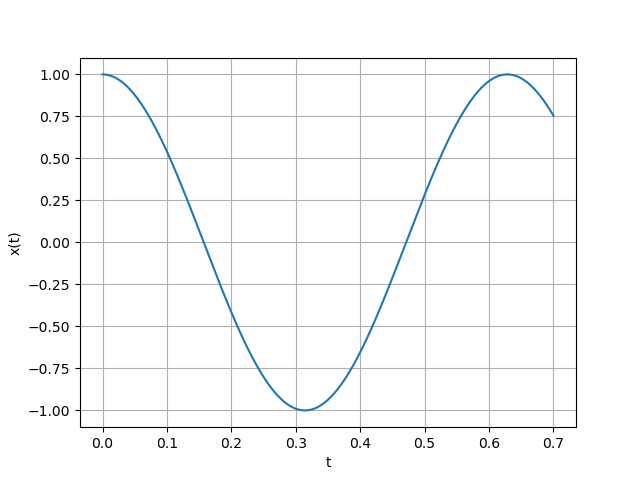
\includegraphics[width = 9cm]{Figure_1}
    Fig. 0. Plot of x\brak{n} \\
    \end{center}
\end{figure}

The ROC of x\brak{n} is defined as the range of values of z for which X\brak{z} will converge where X\brak{z} is the z transform of x\brak{n}.\\
\begin{align}
   \lvert X\brak{z}\rvert = \sum_{n = -\infty}^{\infty}\lvert x\brak{n}z^{-n}\rvert < \infty
\end{align}

By equation \eqref{eq:eq4} :\\
\begin{align}
X\brak{z} &=  7\sbrak{\sum_{n=0}^{\infty}z^{-n}} + 6\sbrak{\sum_{n=0}^{\infty}nz^{-n}} \label{eq:eq7}
\end{align}
The sum $ \brak{\sum_{n=0}^{\infty}z^{-n}} $ will converge only if z is not zero and $ |z^{-1}|< 1 $ as it is forming an infinite GP with common difference $z^{-1}$. 

Observe the second part of the equation \eqref{eq:eq7} or \eqref{eq:eq4} is 6S which was calculated using equation \eqref{eq:eq5} : \\
\begin{align}
    S\brak{1-z^{-1}} &= z^{-1} + z^{-2} + z^{-3} + ... 
\end{align}
The sum S will converge only if z is not 0 and $\lvert z^{-1} \rvert < 1 $ or $ \lvert z \rvert > 1$ as again we obtain an infinite GP with common difference $z^{-1}$.For both the parts of the equation \eqref{eq:eq7}, the ROC is same.

\vspace{4mm}

\large\textbf{Answer} : \normalsize The ROC of X\brak{z} is  $\lvert z \rvert > 1$

\vspace{15mm}

\large\textbf{\brak{ii}} \normalsize The graph of x\brak{n} is :

\vspace{4mm}

\begin{figure}[!ht]
    \begin{center}
    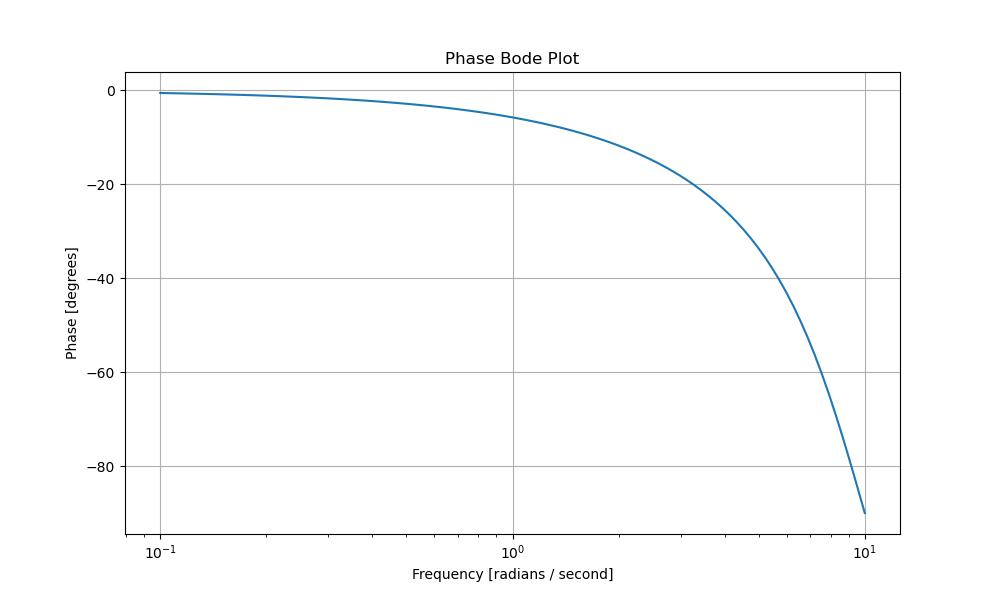
\includegraphics[width = 9cm]{Figure_2}
    Fig. 1. Plot of x\brak{n} \\
    \end{center}
\end{figure}

\FloatBarrier

The ROC of x\brak{n} is defined as the range of values of z for which X\brak{z} will converge where X\brak{z} is the z transform of x\brak{n}.\\
\begin{align}
   \lvert X\brak{z} \rvert  = \sum_{n = -\infty}^{\infty}\lvert x\brak{n}z^{-n}\rvert < \infty
\end{align}

By equation \eqref{eq:eq8} :\\
\begin{align}
X\brak{z} = 18\sbrak{\sum_{n=0}^{\infty}z^{-n}} - \brak{2\frac{1}{2}}\sbrak{\sum_{n=0}^{\infty}nz^{-n}} \label{eq:eq9}
\end{align}
The sum $ \sbrak{\sum_{n=0}^{\infty}z^{-n}}$ will converge only if z is not zero and $\left|z^{-1}\right| < 1$ as it is forming an infinite GP with common difference $z^{-1}$.\\

Observe the second part of the equation \eqref{eq:eq8} or \eqref{eq:eq9} is $-2\frac{1}{2}$S which was calculated using equation \eqref{eq:eq5} : \\
\begin{align}
    S\brak{1-z^{-1}} &= z^{-1} + z^{-2} + z^{-3} + ... 
\end{align}
The sum S will converge only if z is not 0 and $\lvert z^{-1} \rvert < 1 $ or $ \lvert z \rvert > 1$ as again we obtain an infinite GP with common difference $z^{-1}$.For both the parts of the equation \eqref{eq:eq9}, the ROC is same.

\vspace{4mm}

\large\textbf{Answer} : \normalsize The ROC of X\brak{z} is  $|z| > 1$

\end{document}
